%*
%* Seven Kingdoms: Ancient Adversaries
%*
%* Copyright 1997,1998 Enlight Software Ltd.
%* Copyright 2018 Timothy Rink
%*
%* This program is free software: you can redistribute it and/or modify
%* it under the terms of the GNU General Public License as published by
%* the Free Software Foundation, either version 2 of the License, or
%* (at your option) any later version.
%*
%* This program is distributed in the hope that it will be useful,
%* but WITHOUT ANY WARRANTY; without even the implied warranty of
%* MERCHANTABILITY or FITNESS FOR A PARTICULAR PURPOSE.  See the
%* GNU General Public License for more details.
%*
%* You should have received a copy of the GNU General Public License
%* along with this program.  If not, see <http://www.gnu.org/licenses/>.
%*
%*

\chapter{Spies and Espionage}

\index{espionage}

\textgoth{\Huge{U}}sing Spies as \textit{agents provocateurs} is an effective way to help persuade Independent Villagers to acknowledge your rule. And against other Kingdoms, you will have a wide range of missions that your Spies can perform.

\section{Infiltrating Spies}

\begin{wrapfigure}{r}{0.4\textwidth}
	\vspace{-20pt}
	\begin{center}
		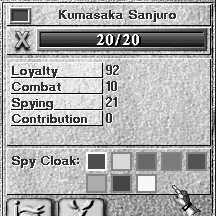
\includegraphics[width=0.4\textwidth]{Ispyinfo} % Original size.
	\end{center}
	\vspace{-15pt}
\end{wrapfigure}

\index{spy!acquiring}

\textgoth{\Huge{Y}}ou acquire Spies by training them in your Villages or by hiring them in Inns.

To infiltrate another Kingdom with a Spy, you will need to set the color of the Spy’s cloak to match that of the targeted Kingdom. Use white for Independent Villages.

To change the Spy’s cloak, select the Spy and then \textbf{Click} on the color of the intended target Kingdom.

Before you make the change though, you will have to make sure that you have toggled the \textbf{Surrender/Sneak Tile} to the correct setting.

\clearpage

\begin{wrapfigure}{r}{0.1\textwidth}
	\vspace{-20pt}
	\begin{center}
		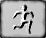
\includegraphics[width=0.1\textwidth]{Tsneak}
	\end{center}
	\vspace{-10pt}
\end{wrapfigure}

% lacking quotation marks? that you have changed cloak colors??

If a Spy is set to Sneak, the enemy Kingdom will not be notified that you have changed cloak colors. This is for when you want to sneak your unit into an enemy Building or Village. You will retain control over your unit when he is toggled to this mode.

\begin{wrapfigure}{r}{0.1\textwidth}
	\vspace{-20pt}
	\begin{center}
		
\includegraphics[width=0.1\textwidth]{Treveal}
	\end{center}
	\vspace{-20pt}
\end{wrapfigure}

% lacking quotation marks? use of "their" and "they" here. Check similar uses.

If a Spy is set to Surrender, the enemy Kingdom will be notified (falsely, of course!) that a unit has betrayed its Kingdom and has joined their own. They may suspect that your unit is in fact a Spy and execute him forthwith, or, as you had hoped, they may take him into their fold and give you a chance of practicing further espionage. When toggled to this mode, you will still retain your ability to move your Spy, but this will risk him being exposed.

You may \textbf{Group Select} several Spies and change their cloaks’ color at the same time.

Spies may not change to a new cloak color if they are near enemy units. They may, however, change back to their original color at any time. This is especially useful when your Spy is a General in command of an enemy Troop. He may then reveal his true colors at a turning point in a battle.

A Spy of yours who has achieved the rank of General will not be able to change his color to that of a third Kingdom and still keep his rank. He will automatically be demoted to common soldier, and it will then be up to the enemy to restore him to his former rank or not.

\begin{wrapfigure}{r}{0.1\textwidth}
	\vspace{-20pt}
	\begin{center}
		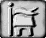
\includegraphics[width=0.1\textwidth]{Tsettle}
	\end{center}
	\vspace{-20pt}
\end{wrapfigure}

% Bold: Settle Cursor ?

To send your selected Spy into a Village, \textbf{Click} on the \textbf{Settle Tile} and then \textbf{Right-Click} the Settle Cursor on the Village.

You may send a Spy into a building with a \textbf{Right-Click} on the building.

\textbf{NOTE}: You cannot send a Spy into a building if it is already full. In this case, you must insert your Spy into a Village and then hope that he is hired by your foe when he builds a new structure.

\subsection{A Spy’s Missions}

\index{spy!missions}

\begin{wrapfigure}{r}{0.1\textwidth}
	\vspace{-20pt}
	\begin{center}
		
\includegraphics[width=0.1\textwidth]{Tspy}
	\end{center}
	\vspace{-20pt}
\end{wrapfigure}

\textgoth{\Huge{W}}hen in a Village or a Building belonging to another kingdom, a Spy will have several possible missions to perform. When that Village or Building is selected, you may toggle these options by \textbf{Clicking} on the \textbf{Spy Tile}.

\subsubsection{Sleep}

\index{spy!sleep mode}

\textgoth{\Huge{I}}n this mode, your Spy is not actively spying. He is instead slowly building up his skill level and quietly insinuating himself into the community. His skill level will increase at a slower pace than if he were performing a more dangerous mission. A Spy cannot be exposed while he is in Sleep mode.

\subsubsection{Sow Dissent}

\index{spy!sow dissent mode}

\textgoth{\Huge{A}}ssign your Spy to this mode when you wish him to drive down the Loyalty of the local Villagers to their King. This will, at the same time, decrease their level of resistance to you and your eventual rule. A Spy may only Sow Dissent among those who are of the same Nationality as the Spy. He will have no effect on units of Nationalities other than his own.

This option is also available when your Spy is working in an enemy Building. It will affect any workers in that Building who are of the same nationality as your Spy.

% NOTE here

If the Villagers revolt against their King, your Spy, who has been Sowing Dissent, will revolt along with them. This will not happen if he is in Sleep Mode.

\subsubsection{Sabotage}

\index{spy!sabotage mode}

\textgoth{\Huge{S}}abotage may be conducted once your Spy has infiltrated an enemy building.

Sabotage in a Mine means that your Spy will cut down the Mine’s rate of Raw Material extraction.

In a Factory and a War Factory, it will result in decreased production speed.

In a Tower of Science, it will slow the speed of research.

Inns and Markets may not be Sabotaged.

If your Spy is employed as the Construction Worker in an enemy structure, he will work to weaken it. This weakness will not be visible to the enemy until the building is attacked. It will then be destroyed much more quickly.

\subsubsection{Bribe}

\index{spy!bribe mode}

\textgoth{\Huge{Y}}our Spies have the ability to bribe enemy units inside firms.

\subsubsection{Why would you want to bribe someone?}

If an enemy worker takes your bribe, he will help you with whatever spying work you are doing in that firm or that Village, multiplying your effectiveness by two. You may, of course, bribe more than one worker.

If your bribe fails, your Spy will be exposed and killed.

The chance of the bribe’s success rests on several things:

\begin{changemargin}{.5cm}{0cm}
The skill level of your Spy.

The amount of money offered.

The loyalty of the unit that you are attempting to bribe.

Your Kingdom’s Reputation.

Your Kingdom’s nationality (The same as the target is better).

Your Spy’s nationality (The same as the target is better).
\end{changemargin}

There is a chance that the unit that you are attempting to bribe is in fact a Spy for another nation or a local in the pay of another nation. If this other nation is your enemy, they will expose and execute your Spy.

\subsubsection{How Do I Offer a Bribe?}

\textbf{\textgoth{\Huge{C}}lick} on a firm that your Spy has infiltrated.

(You will see the \textbf{Spy Tile} confirming that you have a Spy in this firm).

Then \textbf{Click} on the enemy worker that you want to bribe.

\begin{wrapfigure}{r}{0.1\textwidth}
	\vspace{-20pt}
	\begin{center}
		
\includegraphics[width=0.1\textwidth]{Tbribe}
	\end{center}
	\vspace{-20pt}
\end{wrapfigure}

% Spy Icon. Author's voice.

If it is at all possible to bribe this man, you will see the \textbf{Bribe Tile} enabled. \textbf{Clicking} on the \textbf{Bribe Tile} will bring up a list of possible amounts that you can offer to him. This amount will be paid to the man one time only. If the amount is enough, then he will be yours. You will be informed that the bribe has succeeded. From then on, you will see a Spy Icon next to that unit’s picture.

If the bribing amount is not enough, your Spy will be exposed and executed.

If you happen to have more than one Spy in place when you attempt to bribe someone, you will be asked which Spy you want to do the deed. It is best to choose the one with the highest Skill Level.

It is impossible to bribe Kings.

\subsubsection{Stealing Information}

\index{spy!stealing information} % Not a mode?

\begin{wrapfigure}{r}{0.1\textwidth}
	\vspace{-20pt}
	\begin{center}
		
\includegraphics[width=0.1\textwidth]{Tsteal}
	\end{center}
	\vspace{-20pt}
\end{wrapfigure}

\textgoth{\Huge{W}}hen your Spy has infiltrated into any enemy building or Village, you will have the option of stealing information on that enemy Kingdom. To do this, \textbf{Click} on the \textbf{Steal Information Tile}. When you do, you will be presented with a choice of scrolls that your Spy will be able to examine.

\begin{wrapfigure}{r}{0.3\textwidth}
	\vspace{-20pt}
	\begin{center}
		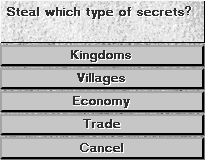
\includegraphics[width=0.3\textwidth]{Isecrets} % Original size.
	\end{center}
	\vspace{-20pt}
\end{wrapfigure}

The scrolls available to your Spy will depend on his Skill Level. Below, you can see what skill levels are needed to view which scrolls:

\begin{changemargin}{.5cm}{0cm}
\textbf{20} - Villages

\textbf{30} - Economy, Trade

\textbf{40} - Kingdoms, Technology

\textbf{50} - Military

\textbf{90} - Espionage \\ % ?
\end{changemargin}

The stealing of this information is the most dangerous thing your Spy can do. It is possible that he will be exposed and executed when the enemy sees that its secrets have been revealed.

Your spy will have the best chance of survival if his skill level is much higher than the level of secrets that he is stealing. If, for instance, your Spy’s skill level is 100 and you give him the task of stealing Trade information (30), he will have a very good chance of survival.

\subsubsection{Assassination}

\index{assassination}
\index{spy!assassination attempts}

\textgoth{\Huge{A}} Spy who has infiltrated an enemy Fort or Seat of Power will have the option of attempting to assassinate the enemy General or King who is in command there.

\begin{wrapfigure}{r}{0.1\textwidth}
	\vspace{-20pt}
	\begin{center}
		
\includegraphics[width=0.1\textwidth]{Tassinate}
	\end{center}
	\vspace{-20pt}
\end{wrapfigure}

To carry out this mission, select the Spy that you wish to use and then \textbf{Click} on the \textbf{Assassination Tile}.

\begin{changemargin}{.5cm}{0cm}
The chance of success will depend upon several factors:

The Hit Points of the target.

The Hit Points of the Spy.

The skill level of the Spy.

The number of other enemy units in the building.

The number of your Spies in the building.

Whether or not there are enemy Counterspies in the building.

A random factor.
\end{changemargin}

If the assassin fails in his mission, he will be immediately exposed and executed. Even if he succeeds, this may still happen, depending upon the other enemy units in the building.

\section{Other Espionage Details}

\subsection{Mobilizing Spies}

\index{spy!mobilization}

\begin{wrapfigure}{r}{0.1\textwidth}
	\vspace{-20pt}
	\begin{center}
		
\includegraphics[width=0.1\textwidth]{Tmobilize}
	\end{center}
	\vspace{-20pt}
\end{wrapfigure}

\textgoth{\Huge{I}}f you wish to take your Spy out of an Independent or an enemy Village, \textbf{Click} on your Spy in the Village’s information area and then \textbf{Click} on the \textbf{Mobilize Tile}. Your Spy will exit the Village, ready for further commands.

\subsection{Capturing Enemy Buildings}

\index{buildings!capturing enemy buildings}
\index{spy!capturing enemy buildings}

\begin{wrapfigure}{r}{0.1\textwidth}
	\vspace{-20pt}
	\begin{center}
		
\includegraphics[width=0.1\textwidth]{Tcapture}
	\end{center}
	\vspace{-20pt}
\end{wrapfigure}

\textgoth{\Huge{A}}t times, you will find that your Spy, or units in your pay, are the only units in an enemy building. If this is the case, you will have one more option. You may Capture the building.

\textbf{NOTE}: Spies may only capture Seats of Power or Forts if they are the commanders there.

The \textbf{Capture Tile} will become visible only when this is possible. If you wish to capture the building, \textbf{Click} on the \textbf{Capture Tile}. The building will change its color to that of your Kingdom.

You may not capture Inns, Markets, or Harbors in this way.

\subsubsection{How Do You Know that a Building Is Empty?}

% COMMA here

Just looking at it may give you some indication. The giant gear in an empty Factory will not be turning, and the Factory will not be spewing smoke. An empty Mine will show no light from inside. The gyroscope on top of an empty Tower of Science will no longer spin. Note that any of these buildings may still be occupied, but producing nothing.

At times, you may defeat and take control of an enemy Village. After your flag is raised over the Village, you will see that the enemy firms that are Linked to that Village will still show the enemy’s colors. If you want to capture these buildings (which may not be empty), select each one and \textbf{Click} on the \textbf{Capture Tile} that will have become visible. There will be no need to send a Spy into them.

\subsubsection{What Happens when the Building Your Spy Is in Is Destroyed?}

If the building is a Fort or a Seat of Power, your Spy will be mobilized and ready for your next command. If it is another type of building, your spy will remain in the local Village. You may access him by \textbf{Clicking} on the \textbf{Spy Tile} when the Village is selected.

\subsection{When Your Spy Becomes a General}

\index{spy!becoming a general}

\textgoth{\Huge{I}}f you have infiltrated a Spy into an enemy Fort, it will sometimes happen that he will be promoted to General. Once your Spy has become a General, you will, when he is in the Fort, have the option of Capturing it. This being done, the soldiers under his command will either join him and your Kingdom or fight against you.

If your General is mobile, you may, at the appropriate time, change his cloak to your Kingdom’s color, thus revealing his true allegiance. At that time, his troop will either join him or fight him.

Once a General has returned his allegiance to you, he will be fully under your control.

\subsection{When Your Spy Becomes a King}

\index{spy!becoming King}

\textgoth{\Huge{A}}t no time does your investment in espionage pay off more than when one of your Spies succeeds to the crown of a foreign Kingdom. This occasion is not without danger however; it all depends upon the level of Loyalty of your Spy.

If the loyalty of your Spy is at a very high level, then it is most likely that he will capture the foreign Kingdom and turn over its rule to you.

If your Spy’s loyalty is somewhat suspect, it is quite likely that he will betray you and rule the captured Kingdom for himself. If the captured Kingdom is more powerful than yours, it will be an added incentive to his betrayal.

\subsection{Disloyal Spies}

\index{spy!disloyal}

\textgoth{\Huge{I}}f the loyalty level of one of your Spies drops too far, he may defect to his targeted nation and become a model citizen. If your Spy is mobile at the time of his defection, he may turn to another Kingdom and move to live there.

\subsection{Executing Spies}

\index{spy!executing}

% Bold the X ?

\textgoth{\Huge{Y}}ou may at any time execute a unit that you suspect of being a Spy by \textbf{Clicking} on the large X to the left of the unit’s blue Hit-Point Bar. If an Executed unit is in fact a Spy from another Kingdom, you and that Kingdom will both be notified that the execution of a Spy has taken place.

% i thought you were just disbanding non spies...

If the unit is not a Spy, your Reputation will decrease by 2\% times the executed unit’s loyalty level.

\subsection{Dropping Spy Identities}

\index{spy!dropping indentity}

\begin{wrapfigure}{r}{0.1\textwidth}
	\vspace{-20pt}
	\begin{center}
		
\includegraphics[width=0.1\textwidth]{Tnospy}
	\end{center}
	\vspace{-20pt}
\end{wrapfigure}

\textgoth{\Huge{A}}t any time, you may order your Spy to lay down his cloak and dagger. He will retain all of his other skills but cease to be in any way associated with spying activities. Do this by \textbf{Clicking} on the \textbf{No Spy Tile} when your Spy is selected.

\subsection{The Cost of Spies}

\index{spy!cost}

\textgoth{\Huge{S}}pies are expensive. When Spies are mobile, you must pay them \$100 per year as their salary and 10 food units per year.

If these Spies have infiltrated another kingdom or an Independent Village, you will no longer have to provide them with food, although you must still pay their salary.

\subsection{Spies and Your Reputation}

\index{spy!effect on reputation} % spelled as "affect" in the original.

\textgoth{\Huge{I}}f one of your Spies is caught in his activities, and subsequently executed, the Reputation of your Kingdom will decrease by three points.

\subsection{Limitations}

\index{spy!limitations}

\textgoth{\Huge{A}}t no time may one of your Spies, in the cloak of another Kingdom, initiate an attack or build any structures unless he is commanded to by the ruler of the Kingdom whose colors he wears. Such actions would immediately expose the spy.

\section{Counterspies}

\index{counterspy}

\textgoth{\Huge{D}}o not feel that you are without defense against these devious operatives. Any Spies that you have trained may be assigned to your own possessions where they will actively work to search for their enemy counterparts.

Their success rate at this will, of course, depend on their skill level and the skills of the enemy agents.

While your Spies are assigned to your firms, they will not just be at work as Counterspies; they will also be picking up skills and contributing to production just as your other workers. It is in this way that you give your Spies those extra skills that they may need before they are sent to infiltrate another kingdom. The higher their secondary skill levels, the more likely it is that another kingdom will welcome them with open arms.

Your Counterspies will also have deceptive loyalty levels. The one that you can see will be their true level. The one that your enemies can see will be false, designed to lure their agents into an offering of a bribe. As soon as this bribe is offered, the enemy Spy will be caught and executed.